\section{Background Information}
\subsection{Histograms of Oriented Gradients}\label{sec:hog}
The most prominent discriminative feature of pedestrians is their shape: limbs, head, and any features with prominent edges \cite{dalal_2005_histograms}. In that regard, HOG features are excellent at pedestrian detection precisely because they prioritize orientation/shape information, unlike other feature descriptors like HaaR wavelets which are colloquially described as “texture features” 
\cite{zia_2015_why}. 
\subsubsection{One Fundamental Property of Images}
At their core, images are matrices that represent pixel intensity values. 
Elements in grayscale image matrices contain a single intensity value, while elements in colored image matrices contain three (one for each color channel). With this definition of an image, it becomes increasingly simple to understand the meaning of "edge".

An edge is a region in which there is a change of intensity. Figure \ref{fig:pixel_intensity} illustrates the changes in pixel intensity by mapping a row's pixel intensity values to a function's output. Observe that an edge is characterized by the gradient of the pixel intensity function. The function's gradient values are greater at the edges/corners of an object, like a pedestrian's limb, rather than homogeneous areas, like background regions. In this way, gradients may highlight the contours of objects and discard noise/texture information, precisely what is needed in pedestrian detection.

\begin{figure}
    \centering
    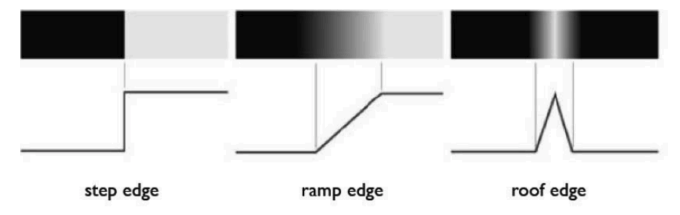
\includegraphics[width=0.75\linewidth]{images/pixel_intensity.png}
    \caption{Representation of the three types of edge that can be found in image analysis.\\Source: \cite{niebles2012edge}}
    \label{fig:pixel_intensity}
\end{figure}

\subsubsection{Gradient Computation}\label{sec:deriv_mask}

In HOG, a derivative mask (also known as a filter or kernel) is used to compute gradient information from an image \cite{dalal_2005_histograms} by performing convolution, the process of adding each element of the image to its local neighbors, weighted by the mask \cite{niebles2012edge}, as shown in equation \ref{eq:convolution}, where $I$ is the image matrix, $K$ the mask's matrix and $k$ - the "radius" of K (the distance from the center element to an edge element). 

\begin{equation}\label{eq:convolution}
    F(x,y) = \sum_{i=-k}^{k} \sum_{j=-k}^{k} I(x+i,y+j) \cdot K(i,j)
\end{equation}

%TODO: Make this discrete convolution equation actually make sense

The authors of HOG found that a simple 1D derivative mask of form $[-1,0,1]$, formally called a central discrete derivative \cite{niebles2012edge}, while being much less computationally expensive than 3x3 Sobel or 2x2 diagonal masks, also performed the best \cite{dalal_2005_histograms}.

Convolution on an image $I$ with the aforementioned 1D mask yields a new image $F_y$ defined in \ref{central_1} and convolution with the transposed, or, in other words, "flipped" over its main diagonal, 1D mask yields an image $F_x$ as defined in \ref{central_2}.

\begin{equation}\label{central_1}
    F_{y}(x_{m},y_{n}) = \frac{ \partial I(x_{m},y_{n}) }{ \partial x } \approx |\ I(x_{m}-1,y_{n})-I(x_{m}+1,y_{n})\ | 
\end{equation}
\begin{equation}\label{central_2}
    F_{x}(x_{m},y_{n}) = \frac{ \partial I(x_{m},y_{n}) }{ \partial x } \approx |\ I(x_{m},y_{n}+1)-I(x_{m},y_{n}-1)\ | 
\end{equation}

Notice however, that $x_m\pm 1$ and $y_n\pm 1$ fall outside $I[0,w-1]\times[0,h-1]$ when $x_m=w-1$ and $y_n=h-1$ respectively. This means that gradient information at image boundaries is lost when using central finite differences for convolution \cite{shidlovskiy_2020_reducing}. The information loss is evident in the \href{https://github.com/scikit-image/scikit-image/blob/main/skimage/feature/_hog.py}{\_hog\_channel\_gradient} where the convolution output at boundary pixels defaults to zero. The nullified boundary pixels may disproportionately impact SVM performance when using smaller detection windows or block sizes, as these zeroed values constitute a larger fraction of the resulting histogram. To address this limitation, this investigation proposes a novel approach that combines central, forward, and backward finite differences \cite{niebles2012edge}.

Figure \ref{fig:finite_differences} displays the kernels of each of the finite differences. Because both forward and backward differences are not anchored around the central pixel, they can be used to yeild the convoluted intensity values of pixels at the top \ref{finite_top} and left \ref{finite_left}, and bottom \ref{finite_bottom} and right \ref{finite_right} edges, respectively.

\begin{figure}
    \centering
    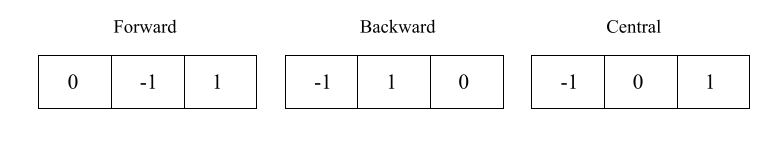
\includegraphics[width=0.75\linewidth]{images/finite_differences.png}
    \caption{Three types of finite differences and their corresponding derivative masks. Source: Image by me}
    \label{fig:finite_differences}
\end{figure}

\begin{equation}
    \label{finite_top}
    F_{x}[x_{m},0] =  | I(x_{m},1)-I(x_{m},0) | 
\end{equation}
\begin{equation}
    \label{finite_left}
    F_{y}[0,y_{n}] =  | I(1,y_{n})-I(0,y_{n}) 
\end{equation}
\begin{equation}
    \label{finite_bottom}
    F_{x}[x_{m},h] =  | I(x_{m},h)-I(x_{m},h-1) 
\end{equation}
\begin{equation}
    \label{finite_right}
    F_{y}[w,y_{n}] =  | I(w,y_{n})-I(w-1,y_{n}) 
\end{equation}

With the convoluted pixel values, or, in a sense, the changes in pixel intensity encoded into both $F_y$ and $F_x$ images, combining them into a single feature map $G$ of gradients, or vectors with an angle $\theta$, is as simple as applying the Pythagorean theorem \cite{shidlovskiy_2020_reducing}, as illustrated in figure \ref{fig:pythagorean}, where $ \text{magnitude} = | G(x_{m},y_{n}) | = \sqrt{ F_{y}(x_{m},y_{n})^2+F_{y}(x_{m},y_{n})^2 }$ and $\theta = \arctan \left( \frac{F_{y}(x_{m},y_{n})}{F_{x}(x_{m},y_{n})} \right) $

\begin{figure}
    \centering
    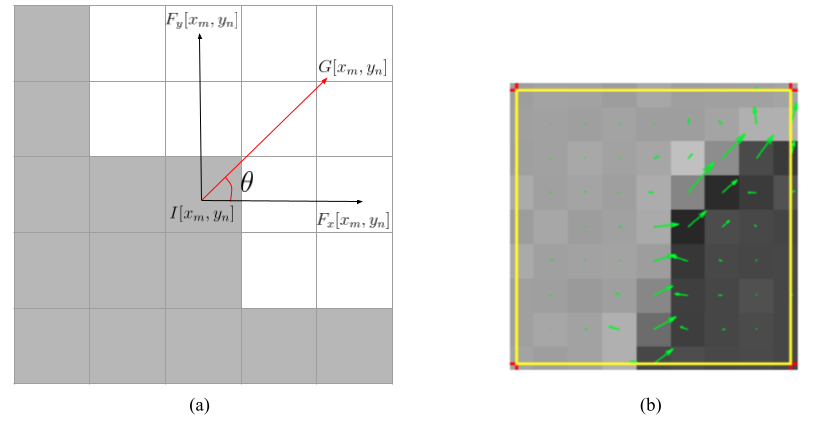
\includegraphics[width=0.75\linewidth]{images/pythagorean.png}
    \caption{(a) Calculation of gradient vector. Source: Image by me (b) Visualisation of gradient vectors. Source: \cite{shidlovskiy_2020_reducing}}
    \label{fig:pythagorean}
\end{figure}

\subsubsection{Orientation Binning}

Orientation Binning hopes to achieve an encoding that is both sensitive to variations in local image content while remaining resistant to miniature changes in pose or appearance. This approach pools gradient orientation information locally, in a similar way that the SIFT feature detector does \cite{lowe_2004_distinctive}.

The process of orientation binning begins with dividing the constructed feature map of gradients into local spatial regions that the authors of the HOG algorithm called cells, as illustrated in figure \ref{fig:cells}.

\begin{figure}
    \centering
    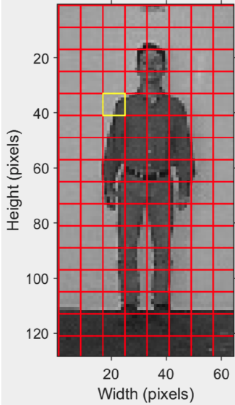
\includegraphics[width=0.3\linewidth]{images/cells.png}
    \caption{A 128x64 image divided into a grid of 8x8 pixel sized cells. Source: \cite{shidlovskiy_2020_reducing}}
    \label{fig:cells}
\end{figure}

Each pixel in a cell contributes to the cell’s local feature vector of size $\omega$, or, as the author put it, a histogram with $\omega$ orientation bins, where the bins are evenly spaced over a 0°-180° “unsigned” gradient, , as shown in figure \ref{fig:histogram_bins} where $\theta$ of each pixel's computed gradient determines which oriented bin, $j$ (from equation \ref{eq:bin}), will receive the computed gradient’s magnitude or vote. 

\begin{equation}
    \label{eq:bin}
    j = \left\lfloor  \left( \frac{\theta \omega}{180°} \right) - \frac{1}{2}  \right\rfloor 
\end{equation}

\begin{figure}
    \centering
    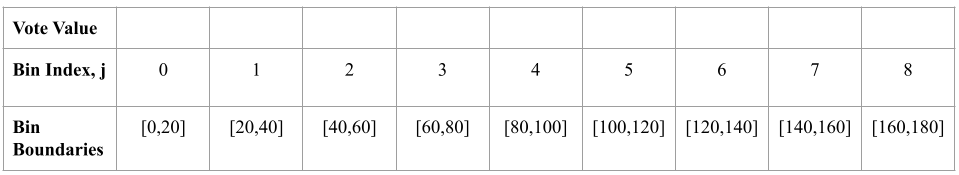
\includegraphics[width=0.75\linewidth]{images/histogram_bins.png}
    \caption{A histogram with 9 equally distributed bins. Source: Image by me}
    \label{fig:histogram_bins}
\end{figure}


While it is also viable to use a “signed” gradient with a range of 0° -360°, it is generally unnecessary to know the sign of a gradient orientation since, as mentioned before, object classification is mainly based on edge detection. Both gradients of orientations 90° and 270° convey the same general trend of changing pixel intensity \cite{shidlovskiy_2020_reducing}. The original HOG authors show that “signed” gradients, while being uninformative, also decrease performance specifically in pedestrian detection \cite{dalal_2005_histograms}, presumably because the wide range of clothing and background colour intensities obfuscate the general shape.

\subsubsection{Block Normalisation}

The magnitude of gradients can vary widely depending on local variations in illumination and foreground-background contrast. The authors of HOG thus found that local contrast normalisation significantly contributes to classifier performance \cite{dalal_2005_histograms}, likely because it allows the classifier to focus on the structure of objects (like edges and gradients) rather than brightness changes. It also ensures contrast invariance, balancing the influence of gradients in both high and low-contrast areas, preventing overemphasis on certain regions. Furthermore, normalization smooths the feature representation, reducing noise and making the extracted features more consistent across the image. By locally adapting to different image regions, normalization helps the classifier identify meaningful patterns and essential details.


Local contrast normalisation is done by grouping the histograms of cells into a single unnormalised descriptor vector, $\vec{f_{b}} = \{ b_{i} \ |\ i=1,2,\dots, c_w \cdot c_h \}$ (where $c_w$ represents the number of pixels in a cell's row and $c_h$ represents the number of pixels in a cell's column). Afterwards, one of the popular block normalisation schemas \cite{dalal_2005_histograms}, namely $\mathrm{L1}$, $\mathrm{L1-sqrt}$, $\mathrm{L2}$ and $\mathrm{L2-hys}$ is applied to $\vec{f_b}$, as illustrated in figure \ref{fig:normalisation}

\begin{figure}
    \centering
    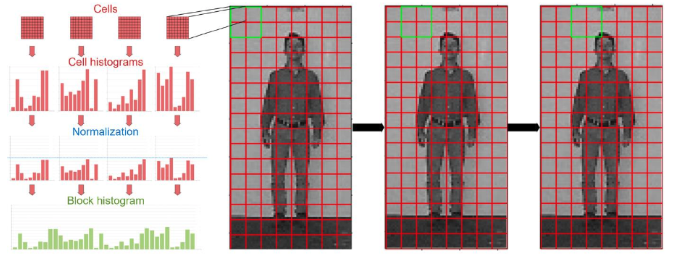
\includegraphics[width=0.75\linewidth]{images/normalisation.png}
    \caption{Construction of histogram blocks of size (2,2). Source: \cite{shidlovskiy_2020_reducing}}
    \label{fig:normalisation}
\end{figure}

One essential feature of grouping cell histograms into blocks is that the blocks themselves may overlap. Depending on the stride with which the block window moves, the horizontal and vertical overlaps will be $(1-\frac{\text{block width}}{\text{horizontal block stride}})\%$ and $(1-\frac{\text{block height}}{\text{vertical block stride}})\%$ respectively. While normalising the same histograms in different block contexts may seem redundant, the authors of HOG found that the increased number of descriptor vectors $\vec{f_b}$ significantly improved performance \cite{dalal_2005_histograms}.

%TODO: Explain WHY it improved performance

\subsubsection{Feature Vector Dimensionality}\label{sec:feature_vector_dimensionality}

A sliding detection window is essential for object detection tasks like pedestrian classification because it allows the classifier to systematically examine all parts of the image at various positions and scales. Objects of interest, such as pedestrians, can appear at different locations, sizes, and orientations within an image, making it crucial to have a method that can effectively search across the entire image space. The sliding detection window of dimensions  $W_h$ and $W_w$ scans the image in a grid-like fashion, shifting over both horizontal and vertical axes. At each location, the window encompasses a region of interest containing a dense grid of overlapping blocks.

As the window moves across the image, the feature descriptors $\vec{f_b}$ within each block's region are computed, normalized, and combined into a larger feature vector, $\vec{L}$, as illustrated in figure \ref{fig:hog_pipeline}. The vector $\vec{L}$, representing the entire sliding window at that position, is used as input to the linear Support Vector Machine classifier to decide whether the window contains a pedestrian or not. 

\begin{figure}
    \centering
    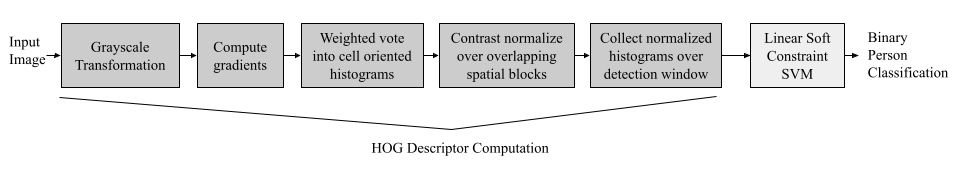
\includegraphics[width=1\linewidth]{images/HOG Pipeline.png}
    \caption{An overview of the HOG feature extraction chain. Source: Adapted by me from \cite{dalal_2005_histograms}}
    \label{fig:hog_pipeline}
\end{figure}

The dimensionality, $d$, of the vector $\vec{L}$ in essence describes the the total number of individual features, where each feature represents the direction of gradients in a specific region of the image. Formally, it is said that the vector $\vec{L}$ belongs in a feature space of $d$ dimensions ($\vec{L} \in \mathcal{R}^{d}$). The higher the dimensions of this space, the more information a model has to distinguish between a pedestrian and the background or a humanoid silhouette. 

If we were to restrict the possible spatial block region's horizontal, $b_w$, and vertical, $b_h$, dimensions to even numbers, it could be easily expressed that the center coordinates, $x$ and $y$, of any block are bounded within $\left[ \frac{b_w}{2}; \frac{W_w}{c_w} - \frac{b_w}{2}\right]$ and $\left[ \frac{b_h}{2}; \frac{W_h}{c_h} - \frac{b_h}{2}\right]$ sets of cell values, respectively, as illustrated in figure \ref{fig:center_coords}

\begin{figure}
    \centering
    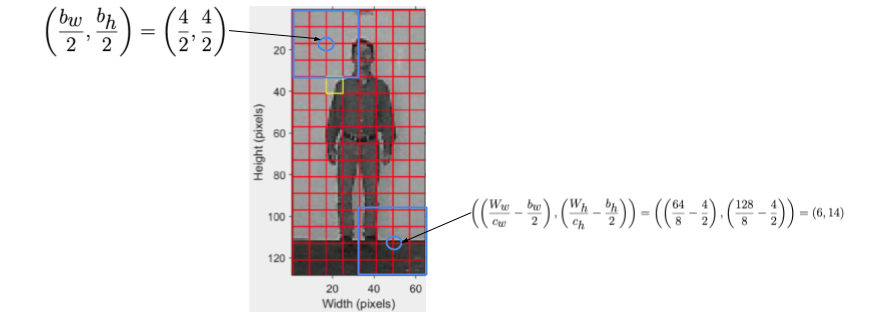
\includegraphics[width=1\linewidth]{images/Center Coordinates.png}
    \caption{A 128x64 sized image with cells that contain 8x8 pixels and blocks that contain 4x4 cells. The top left-most and bottom-right most block coordinates are each expressed using the aforementioned bounds. Source: Adapted by me from \cite{shidlovskiy_2020_reducing}}
    \label{fig:center_coords}
\end{figure}

Since the dimensions of each feature descriptor $\vec{f_b}$ are defined by the number of cells that comprise that descriptor ($c_w\cdot c_h$) and the number of orientation bins ($\omega$) that each cell's histogram contains, and since the total number of descriptors combined to $\vec{L}$ is equal to the number of blocks (with horizontal and vertical strides of $s_w$ and $s_h$) in the window, it follows that the dimensionality $d$ of the resultant feature vector $\vec{L}$ is a combination of cell size, the number of orientation bins, block size, block stride values, and the size of the window itself, as shown in equation \ref{vector_dimensions}

\begin{equation}
    \label{vector_dimensions}
    \begin{split}
    d &= \left\lfloor \frac{\frac{W_w}{c_w}-2\cdot\frac{b_w}{2}+1}{s_w} \right\rfloor\left\lfloor \frac{\frac{W_h}{c_h}-2\cdot\frac{b_h}{2}+1}{s_h} \right\rfloor\cdot b_w b_h\omega \\ &= \left\lfloor  \frac{W_w- c_w(b_w-1)}{s_w c_w}  \right\rfloor \left\lfloor   \frac{W_h -c_h(b_h +-1)}{s_h c_h} \right\rfloor b_w b_h\omega
    \end{split}
\end{equation}

\subsection{Supervised Machine Learning}\label{sec:supervised_ml}

Machine Learning (ML), on a surface level, is the study of algorithms that are designed to produce outputs without an explicit instruction set generated by a person but rather with reference to the patterns or correlations found in data \cite{what_is_ml}. 

In that respect, Supervised ML algorithms are a subset of ML algorithms which attempt to make predictions from data \cite{supervised_learning}. Such algorithms rely on labeled training datasets, or data sets which provide the correct outputs that an algorithm should produce for each input data point \cite {supervised_learning}. 

Supervised ML applications include classifiers, such as a pedestrian detection program, which learn from previously annotated data in the hope of predicting the "class" to which future input data will belong. \cite{derek_2020_svm}. For example, a good pedestrian classifier should be able to predict whether an image's window belongs to the class of windows that contain a pedestrian or to the class of windows that do not contain a pedestrian.

Formally, classifier training data is defined as $D=\{ (x_{1},y_{1}),\dots,(x_{n},y_{n}) \}$, where each $x$ which belongs to a $d$-dimensional feature space \cite{supervised_learning} ($x\in \mathcal{R}^d$)  and each $y$ belongs to a label space \cite{supervised_learning} ($y\in \mathcal{C}$). A label space is simply the set of the possible labels or classes to which a data point might belong. Given that the goal of this investigation is to construct such a descriptor which optimises the detection of a pedestrian, the label space contains two labels $+1$ and $-1$, as required for binary classification \cite{cornell_svm}. Also notice that $x$, a data point in $D$, matches the definition of a fully constructed HOG feature vector $\vec{L}$, meaning that whenever the dimensionality of $\vec{L}$ changes, as defined in section \ref{sec:feature_vector_dimensionality}, a new classifier model will have to be trained on a data set which contains points that belong in the appropriate dimension space.

\subsection{Support Vector Machines}


Support Vector Machines (SVM) is one of the most popular supervised machine learning (ML) algorithms \cite{chang_lin_2011_libsvm} \cite{derek_2020_svm}. While there are many types of ML algorithms that can perform classification, such as decision trees \cite{cornell_decision_trees}, naïve bayes \cite{cornell_naive_bayes} and deep learning networks \cite{cornell_nn}, SVMs have become widely adopted because of how effectively they  handle high dimensional feature spaces \cite{ng_support}. In classification SVMs are highly regarded for their versatility that extends across multiple data science scenarios \cite{derek_2020_svm}, like brain disorders research \cite{derek_2020_svm}, neuroimaging \cite{svm_mri} and, of course, pedestrian detection \cite{dalal_2005_histograms}.

An SVM decision function can be precisely described as the optimal boundary, or hyperplane (defined through an optimised weight, $w$, and bias, $b$, as a set of points such that $\mathcal{H}=\{ x|w^\top x + b = 0 \}$ \cite{cornell_svm_notes}), that serves to separate, or classify, data points belonging to one class from another based on the data points' features \cite{derek_2020_svm}. The SVM model differs from other approaches that seek to find such a seperating hyperplane (for example, the Perceptron algorithm \cite{cornell_perceptron}) in that the SVM attempts to find a hyperplane with the maximum margin between data points closest to the plane (which are called support vectors) \cite{ng_support}, as illustrated in figure \ref{fig:hyperplane} where the hyperplane is a straight line with a weight that is orthogonal to the line and a bias that is the $y$ intercept of the line. 

\begin{figure}
    \centering
    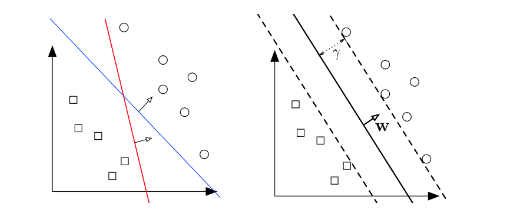
\includegraphics[width=0.75\linewidth]{images/hyperplane.png}
    \caption{A 2 dimensional space, where each data point has 2 features (one abscissa and one ordinate component) (Left:) Two different separating hyperplanes for the same data set (the multiple possibles hyperplanes of, for example, the perceptron algorithm). (Right:) The maximum margin hyperplane (the only possible hyperplane of the SVM algorithm). Source: \cite{cornell_svm_notes}}
    \label{fig:hyperplane}
\end{figure}

A hyperplane with the maximum possible margin between its support vectors is incredibly useful as it increases the likelihood of producing a generalized classifier, which can accurately seperate unseen data points \cite{cornell_svm}. By expressing the distance between any point and that point's projection in the hyperplane, as illustrated in figure \ref{fig:hyperplane_geometry}, with the two variables that define the hyperplane itself (the weight and the bias), we get a definition of the margin, $\gamma$ in \ref{margin_expr} \cite{cornell_svm_notes}

\begin{equation}\label{margin_expr}
    \gamma(w,b)=\min_{x\in D} \frac{|w^\top x + b|}{||w||_{2}}
\end{equation}

\begin{figure}
    \centering
    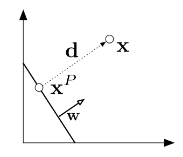
\includegraphics[width=0.35\linewidth]{images/hyperplane_geometry.png}
    \caption{The projection of a data point onto the hyperplane. Source: \cite{cornell_svm_notes}}
    \label{fig:hyperplane_geometry}
\end{figure}

With the expression in \ref{margin_expr}, the abstract goal of finding the hyperplane "of best fit" becomes a very concrete optimization problem which seeks to obtain such a weight $w$ and bias $b$ that the margin $\gamma$ is maximised while maintaining the constraint that the data points of each class must lie on the correct sides of the hyperplane. Mathematically, this constraint is the inequality in equation \ref{hyper_inequality} \cite{ng_support}, since plugging in any data point $x_i$ into the the equation $w^\top x +b$ will yield an output that is either $\ge 0$ or $\le 0$. For positive outputs, the data point (or the input into the equation) will be above the hyperplane, $\mathcal{H}$, so we should expect that data point's label $y_i$ to also be positive, and for negative outputs it, where $x_i$ is below $\mathcal{H},$ a negative label should be expected.

\begin{equation}\label{hyper_inequality}
y_{i}(w^\top x_{i}+b)\ge 0 \quad 
\end{equation}
%TODO: Should I expand more on the concrete form of how this optimization problem looks?

\subsubsection{Soft SVM Constraints}\label{sec:soft_constraint_svm}

Traditionally obtaining the largest possible margin $\gamma$ would be a quadratic programming problem \cite{quadratic_programming} (as the goal of maximising $\gamma$ is primarily anchored around minimizing $||w||_{2}$ from the equation in \ref{margin_expr} with the linear constraint in \ref{hyper_inequality}). While an SVM model's hyperplane with the hard constraint in \ref{hyper_inequality} could, in theory, be found found using either QCQP \cite{cornell_svm_notes} or SMO \cite{chang_lin_2011_libsvm} algorithms, in practice pedestrian datasets are incredibly noisy, as mentioned in section \ref{sec:introduction}, while also containing humanoid figures which closely approximate the features of a pedestrian \cite{inria_improved}, as visualized in figure \ref{fig:manequin_features}. Because of noise and obfuscation in real world pedestrian data, an SVM with a hard linear constraint would fail to compute the optimal hyperplane as there would be a significant number of outliers or data points which share features common to both classes, as illustrated in figure \ref{fig:outliers}. Instead, in the hope of finding a hyperplane that achieves the best realistically possible classification accuracy, an SVM with a soft constraint, which does allow for some degree of error while maximising $\gamma$, ought to be used \cite{dalal_2005_histograms} \cite{cornell_svm_continued}.

\begin{figure}
    \centering
    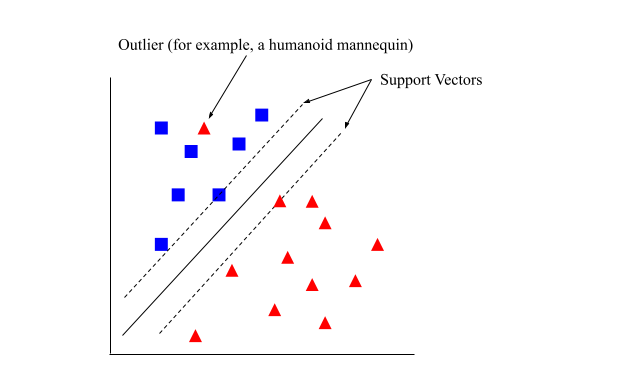
\includegraphics[width=0.75\linewidth]{images/outliers.png}
    \caption{A Data set with two classes and an outlier. Source: Image by me}
    \label{fig:outliers}
\end{figure}

\begin{figure}
    \centering
    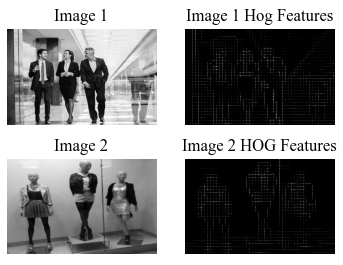
\includegraphics[width=0.75\linewidth]{images/features.png}
    \caption{(Image 1: ) An Image containing three people/pedestrians in a building. Source: \href{https://www.istockphoto.com/photo/business-people-taking-a-break-gm639259132-115111535}{istockphoto.com} (Image 2:) An Image containing three mannequins in a store window. Source: \href{https://theshopcompany.com/blog/Mannequins_and_Dressforms_Who_Uses_What}{theshopcompany.com} (Image 1 and 2 Hog Features): Computed HOG Features of Image 1 and Image 2. Source: Image by me}
    \label{fig:manequin_features}
\end{figure}

% TODO: Will I even be able to explain how to maximise the margin?



